
\documentclass{cgsblatt}


\usepackage[super]{nth}
\usepackage{mathtools}

\DeclarePairedDelimiter\ceil{\lceil}{\rceil}
\DeclarePairedDelimiter\floor{\lfloor}{\rfloor}

\let\theexercise 1
\setcounter{section}{0}

\title{Advanced Programming in C++}
\subtitle{Assignments \# \theexercise}
\date{Winter Term 2016/17}
\author{Prof. Dr. Jürgen Döllner}
\makeatletter
\let\thesubtitle\@subtitle
\makeatother

\begin{document}

\maketitle

\section*{Objectives}
In your first assignments you will learn how to:
\begin{itemize}
\setlength{\parskip}{0pt}
\item start programming in C++;
\item use the command line as basic tool and environment for programming;
\item use CMake for the program building process;
% \item use git as version control system to manage your source code;
\item design and implement text-oriented low-level features;
\item apply some fundamental components of the C++ Standard Library (\emph{std}).
\end{itemize}

For your programming tasks, you should not use common programming IDEs; 
perform your tasks \emph{in the shell}, i.e., using the command line and its tools, 
e.g., the command-line editor \enquote{vim}.


\section{\enquote{Hello, World!}}

\blueify{File:} 
\lstinline|greet_world.cpp|

\blueify{Description:} 
Implement a variant of the famous \enquote{Hello, World!}
using I/O streams from the \emph{std}.

\begin{itemize}\setlength{\parskip}{4pt}

    \item If a command line argument is handed over, 
    it replaces the word \enquote{World} in the output message. 
    \item If two arguments are handed over, they are printed separated by an \enquote{and}
    \item If more than two arguments are handed over, 
    they are printed separated by commas,
    but the last argument is preceded with \enquote{, and}.
    \item There is no need to repack the arguments into \lstinline|std::string| objects; 
    just take the character pointers as provided as arguments of the \lstinline|main| function. 
    \item Intercept and review the assembler output that the compiler generates. 

\end{itemize} 

\blueify{Artifacts:}
\begin{enumerate}
	\item \redify{\lstinline|greet_world.cpp|} : Source code of the solution.
	\item \redify{\lstinline|greet_world.asm|} : Generated assembler code for your system.
\end{enumerate}

\blueify{Example:}

\hspace{\leftmargin}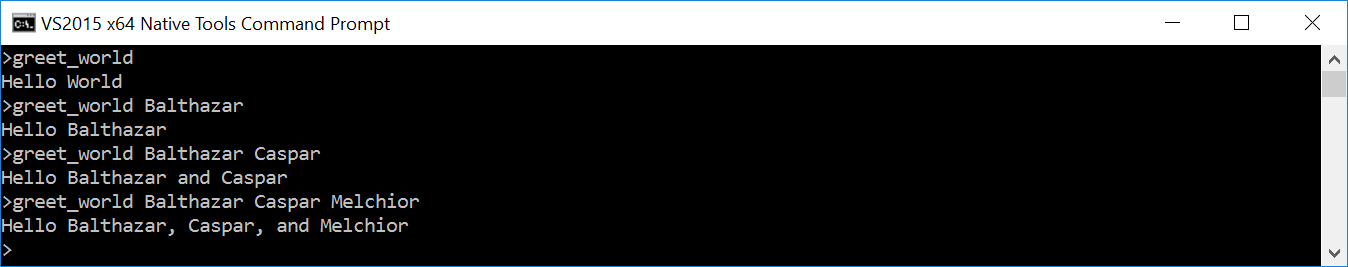
\includegraphics[width=\linewidth-\leftmargin]{greet_world}

\blueify{Objectives:} 
C++ program building process, includes, compiler options. 



\section{Provider Information Library}

\blueify{Files:} 
\lstinline|provider.cpp, provider.h, providerlibtest.cpp|

\blueify{Description:} 
Implement a C++ library that allows access to the library's provider name 
and, optionally, the creation date and time of the library. 
The library should 

\begin{itemize}\setlength{\parskip}{4pt}

\item declare a function \lstinline|std::string providerInfo(bool date = false)|
in a header file (provider.h); 
\item implement the corresponding function (provider.cpp); take your name(s) as provider name and use appropriate C++ built-in macros for build date and time;
\item generate a library that can dynamically linked;
\item handle symbol visibility explicitly in your library headers (i.e., handle \lstinline|dllimport| and \lstinline|dllexport| on Windows as well as \lstinline|__attribute__ ((visibility ("default")))| on unixoid systems);
\item compile \lstinline|providerlibtest.cpp| without any modifications to the source code to test your library. 

\end{itemize}

\blueify{Artifacts:}
\begin{enumerate}
	\item \redify{\lstinline|provider.cpp|, \lstinline|provider.h|} : Source code of the solution.
   	\item \redify{\lstinline|provider_make.txt|} : The full compilation command used for generating the library and compilation of the test and linkage of the library for at least one platform.
\end{enumerate}

\blueify{Example:}

\hspace{\leftmargin}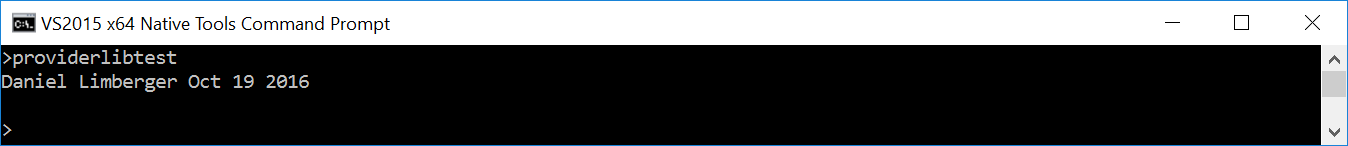
\includegraphics[width=\linewidth-\leftmargin]{providerlibtest}

\blueify{Objectives:} 
C++ library building process and usage; predefined macros of C++. 




\section{Pipeline-Based Email Address Validation}

\blueify{Files:} 
\verb|validate_emails.cpp, addressdata.txt |

\blueify{Description:} 
Implement a program that 
reads a variable number of text tokens from standard input (separated by a newline), 
tests for each token whether it represents a valid email address, sorts the valid email addresses
and writes them to the standard output. 

\begin{itemize}
\setlength{\parskip}{4pt}
\item The program can be used in a pipeline, 
i.e., a sequence of processes chained together by their standard streams, 
so that the output of each process (\lstinline|std::cout|) 
feeds directly as input (\lstinline|std::cin|) to the next one. Example: \\

\begin{lstlisting}[style=Bash]
cat addressdata.txt | validate_emails > emaildata.txt
\end{lstlisting}\medskip

or on Windows, respectively:

\begin{lstlisting}[style=Bash]
type addressdata.txt | validate_emails > emaildata.txt
\end{lstlisting}\medskip

\item The tokens should be represented by \texttt{std::string} objects.
\item To store and sort valid email addresses, 
use an appropriate \texttt{std} container with the element type \lstinline|std::string|.
\item To identify email addresses, 
use regular expressions (e.g., \lstinline{std::regex_match}), e.g., \\
\lstinline|^[A-Z0-9._%+-]+@[A-Z0-9.-]+\.[A-Z]{2,4}$|
\item Email addresses should be sorted 
(1) by ascending order of their domain 
and (2) by ascending order of their name.
\item All non-email tokens are ignored and skipped (in default mode; see below). 
\item Support multiple modes of this program:
\begin{enumerate}
	\item Filter invalid email addresses and print out valid ones with the sorting algorithm defined above (explicitly turned-on with \lstinline{--print-valid} command line argument), and
	\item Filter valid email addresses and print out invalid ones with their input order (turned on with \lstinline{--print-invalid} command line argument).
\end{enumerate}
\end{itemize}

\blueify{Artifacts:}
\begin{enumerate}
	\item \redify{\lstinline|validate_emails.cpp|} : Source code of the solution.
	\item \redify{\lstinline|valid_addresses.txt|} : All valid email addresses of \lstinline|addressdata.txt| sorted as defined above.
	\item \redify{\lstinline|invalid_addresses.txt|} : All invalid email addresses of \lstinline|addressdata.txt| in input-order.
\end{enumerate}

%\blueify{Example:}
%\hspace{\leftmargin}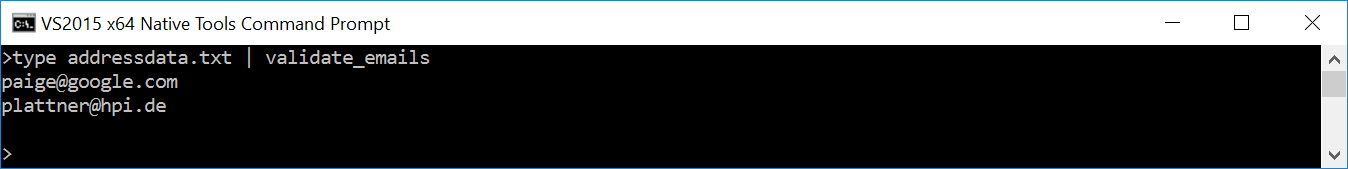
\includegraphics[width=\linewidth-\leftmargin]{validate_emails} % this is not a valid output anymore

\blueify{Objectives:} 
Standard input/output; Unix-like pipelines; strings, sorting and regular expressions. 



\section{Word Histogram}

\blueify{Files:} \verb|count_words.cpp|, \verb|hgg.txt|

\blueify{Description:} 
Implement a program that 
reads the text file \texttt{hgg.txt} (\enquote{The Hitchhiker's Guide to the Galaxy}) 
and counts the occurrences of all distinct words. The occurrences are sorted by frequency and printed to \lstinline|std::cout|.
By conducting a manual review of the output, which are the top four main protagonists in the text?

\begin{itemize}
\item A \emph{word} is a sequence of (one or more) 
case-insensitive alphanumerical characters including apostrophes.
\item \lstinline|regex| and \lstinline|sregex_token_iterator| can be used to identify words.
\item The top \lstinline|n| words
with highest occurences are printed to the standard output.
\item \lstinline|n| is adjustable by an optional command line argument (\lstinline|n = 32| by default).
\item The output has to be formatted into two columns (first is right aligned, second is left aligned). 
\item Use appropriate \lstinline|std| containers to keep the implementation simple. 
\end{itemize}

\blueify{Artifacts:}
\begin{enumerate}
	\item \redify{\lstinline|count_words.cpp|} : Source code of the solution.
	\item \redify{\lstinline|hgg_protagonists.txt|} : Order and frequency of the four main protagonists of \enquote{The Hitchhiker's Guide to the Galaxy}.
\end{enumerate}


\blueify{Example:}

\hspace{\leftmargin}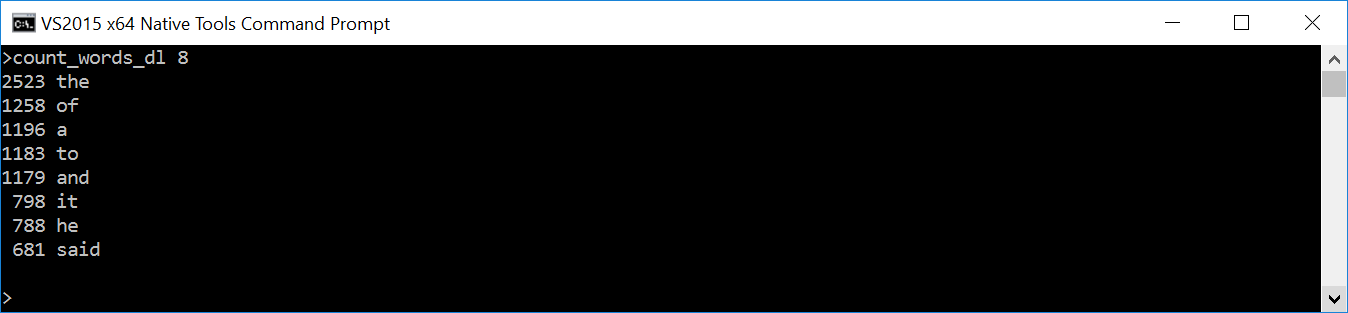
\includegraphics[width=\linewidth-\leftmargin]{count_words}


\blueify{Objectives:} 
String I/O, regular expressions, associative maps. 


\pagebreak
\section*{Instructions}

\paragraph{Pair Programming}
On these assignments, 
you are encouraged (not required) to work with a partner 
provided you practice pair programming. 
Pair programming \enquote{is a practice in which two programmers work side-by-side at one computer, continuously collaborating on the same design, algorithm, code, or test.}
One partner is driving (designing and typing the code) 
while the other is navigating (reviewing the work, identifying bugs, and asking questions). 
The two partners switch roles every 30-40 minutes, and on demand, brainstorm.

\paragraph{Cross-Platform}
The assignments can be solved on all major platforms (i.e., Windows, Linux, macOS).
The evaluation of submitted assignments can be carried out on any of these platforms. 
All results are required to be cross-platform, that is, they compile successfully and run indifferently with respect to their input and output.

\paragraph{Upload Results}
All described artifacts are submitted to the course moodle system \url{https://moodle.hpi3d.de/mod/assignment/view.php?id=2678} as a zipped archive with the 
following naming convention: \verb|assignment_1_matrikNr1.zip| or \verb|assignment_1_matrikNr1_matrikNr2.zip| whether or not pair programming was applied. 
Compiled, intermediate, or temporary files should not be included (\lstinline|*.obj, *.pdb, *.ilk, *.ncb|).
If pair programming is used, the results are turned in only once. 
The assignments \#\theexercise{} are due to the next tutorial on \redify{November \nth{2}, 9:15 a.m.}

\paragraph{Violation of Rules} a violation of rules results in grading the affected assignments with $0$ points.
\begin{itemize}
\item Writing code with a partner without following the pair programming instructions listed above (e.g., if one partner does not participate in the process) is a serious violation of the course collaboration policy.
\item Plagiarism represents a serious violation of the course policy. 
\end{itemize}


\end{document}
